\documentclass[tikz,border=2pt]{standalone}
\usepackage{amsmath}
\usepackage{pgfplots}
\pgfplotsset{compat=1.18}

\begin{document}
% |x| is continuous on [-1,1] but has a corner, so no Taylor series helps; still, polynomials
% of growing degree (least-squares fits) come uniformly closer and closer to it.
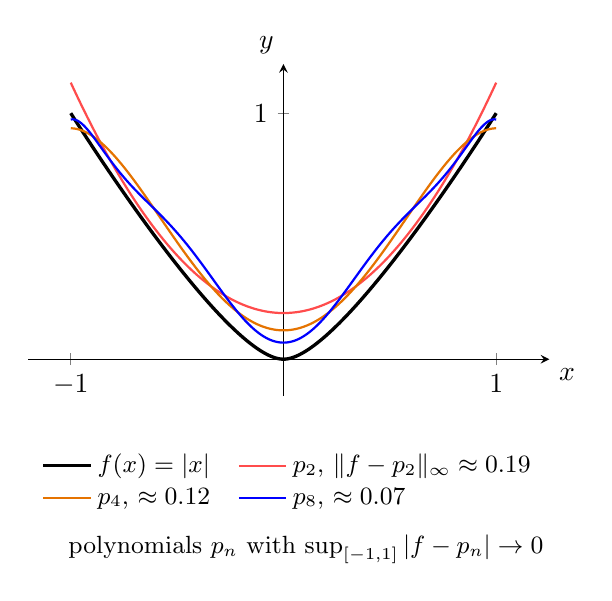
\begin{tikzpicture}
	\begin{axis}[
		axis lines=middle,
		xmin=-1.2, xmax=1.25,
		ymin=-0.15, ymax=1.2,
		xtick={-1,1}, ytick={1},
		xlabel={$x$}, ylabel={$y$},
		xlabel style={below right}, ylabel style={above left},
		samples=200, smooth, clip=false,
		width=8.2cm, height=5.8cm,
		legend style={draw=none, fill=none, font=\small, at={(0.5,-0.14)}, anchor=north, legend columns=2, /tikz/every even column/.append style={column sep=8pt}}, legend cell align=left
		]
		\addplot[very thick, black, domain=-1:1, samples=3] {abs(x)};
		\addlegendentry{$f(x)=|x|$}
		\addplot[thick, red!70, domain=-1:1] {0.1877+0.9363*x^2};
		\addlegendentry{$p_2$, $\|f-p_2\|_\infty\approx0.19$}
		\addplot[thick, orange!90!black, domain=-1:1] {0.1173+1.6386*x^2-0.8173*x^4};
		\addlegendentry{$p_4$, $\approx0.12$}
		\addplot[thick, blue, domain=-1:1] {0.0674+2.9572*x^2-6.3917*x^4+7.6513*x^6-3.31*x^8};
		\addlegendentry{$p_8$, $\approx0.07$}
	\end{axis}
	\node[anchor=north, font=\small] at ([yshift=-2pt]current axis.outer south) {polynomials $p_n$ with $\sup_{[-1,1]}|f-p_n|\to0$};
\end{tikzpicture}
\end{document}
